% Auto-generated from independently audited v8 evidence e932c88a73fe7fa9e3b70b487d798a1504994e3ae6841c26ff335070cbb2ffff.
% Prepared fragment only: paper integration remains an explicit reviewed action.
\begin{figure*}[t]
  \centering
  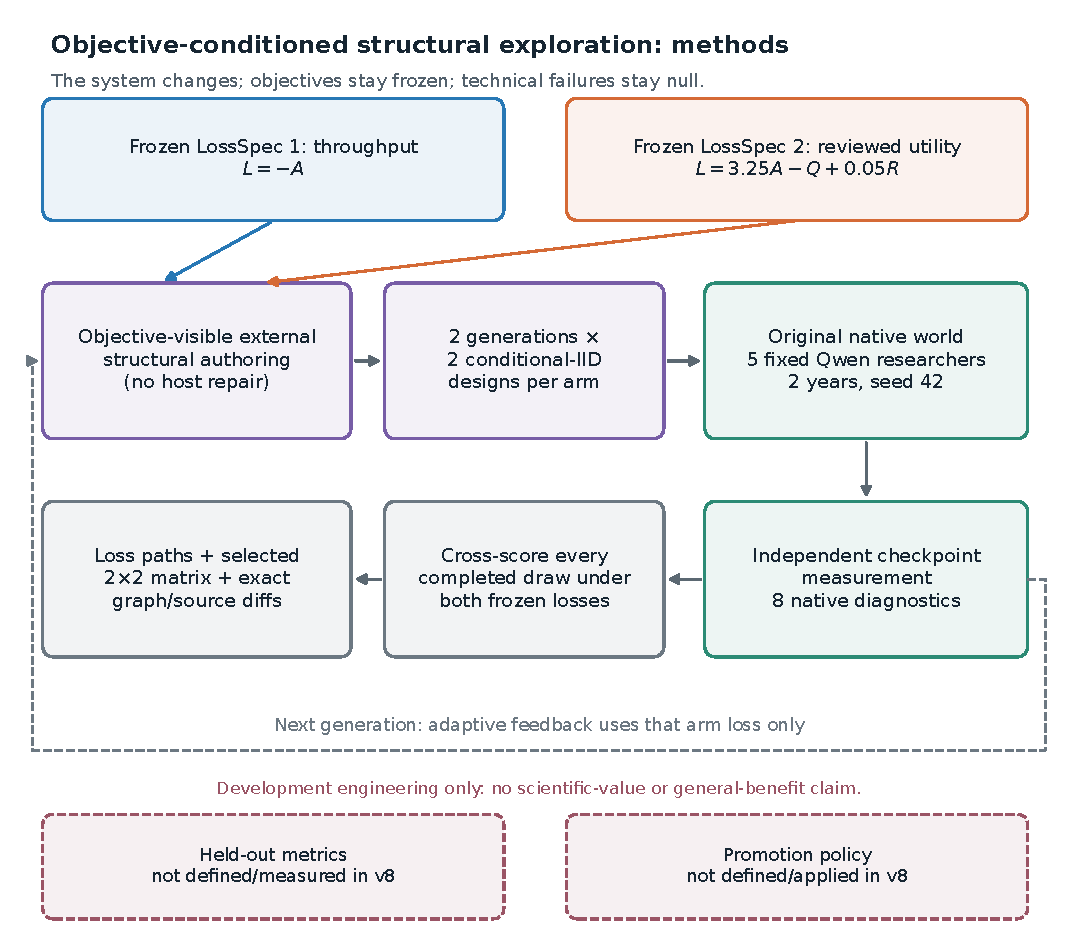
\includegraphics[width=\textwidth]{figures/native-objective-structure-v8-methods.pdf}
  \caption{Preregistered two-objective native structural exploration. The system is optimized while each LossSpec remains frozen. Held-out metrics and promotion are outside this development-engineering pilot.}
  \label{fig:native-objective-structure-v8-methods}
\end{figure*}

\begin{figure*}[t]
  \centering
  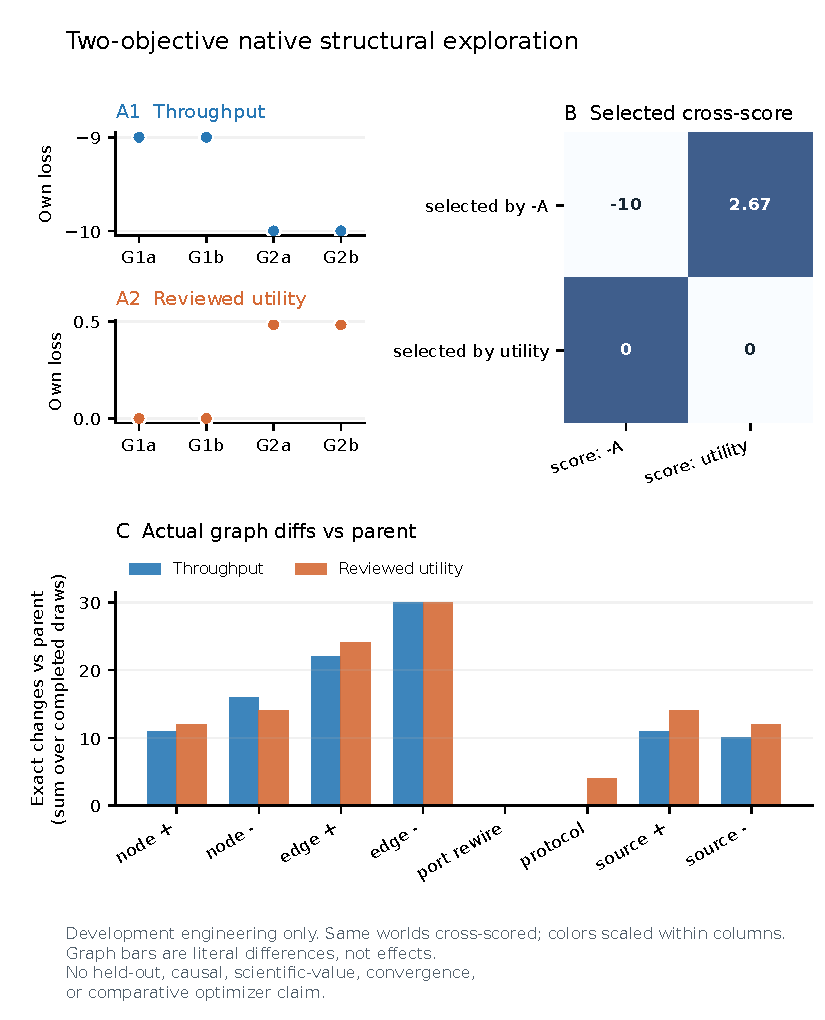
\includegraphics[width=\textwidth]{figures/native-objective-structure-v8.pdf}
  \caption{Audited development loss paths, cross-objective scores of the two selected representatives, and literal graph/source differences. Cross-scores reuse the same worlds and are not independent replications.}
  \label{fig:native-objective-structure-v8-results}
\end{figure*}

\begin{table}[t]
\centering
\caption{Selected-system development cross-scores (lower is better within a column; objectives have different units).}
\label{tab:native-objective-structure-v8-crossscores}
\begin{tabular}{lrr}
\toprule
Selection objective & $-A$ & $3.25A-Q+0.05R$ \\
\midrule
$-A$ & -10 & 2.667 \\
Reviewed utility & 0 & 0 \\
\bottomrule
\end{tabular}
\end{table}

\paragraph{Scope.} These are objective-conditioned development-engineering observations. Observed loss changes do not establish held-out, causal, scientific-value, optimizer-convergence, or generalized institutional benefit. Technical failures remain null rather than numerical penalties.
